
A)
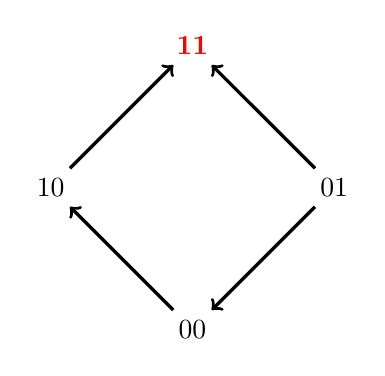
\begin{tikzpicture}
[thick, color=black,scale=0.9]
%[scale=0.6, auto=left,every node/.style={circle, draw,
%thick,outer sep=5pt}]
  \node (n1) at (4,0) {00};
  \node  (n2) at (2,2)  {10};
  \node   (n3) at (6,2)  { 01};
  \node [color=red] (n4) at (4,4) {\bf 11};
  \foreach \from/\to in {n2/n4,n3/n4,n1/n2,n3/n1}
  \draw[very thick] [-> ](\from) -- (\to);
\end{tikzpicture}
B)
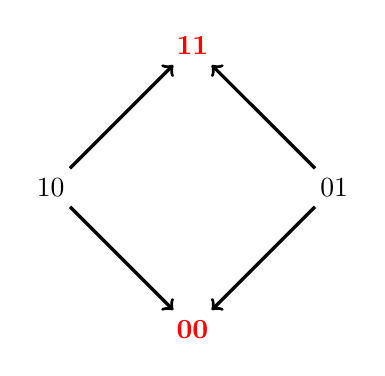
\begin{tikzpicture}
[thick, color=black,scale=0.9]
%[scale=0.6, auto=left,every node/.style={circle, draw,
%thick,outer sep=5pt}]
  \node [color=red]  (n1) at (4,0) {\bf 00};
  \node  (n2) at (2,2)  {10};
  \node   (n3) at (6,2)  { 01};
  \node [color=red] (n4) at (4,4) {\bf 11};
  \foreach \from/\to in {n2/n4,n3/n4,n2/n1,n3/n1}
  \draw[very thick] [-> ](\from) -- (\to);
\end{tikzpicture}
 C)
 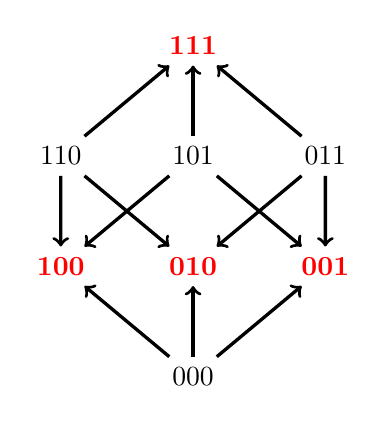
\begin{tikzpicture}
[very thick, color=black,->,scale=1.4]
\node (n0) at (0,0) {000};
\node  [color=red] (n1) at (1.2,1) {\bf 001};
\node  [color=red] (n2) at (0,1) {\bf 010};
\node (n3) at (1.2,2) {011};
\node  [color=red] (n4) at (-1.2,1) {\bf 100};
\node (n5) at (0,2) {101};
\node (n6) at (-1.2,2) {110};
\node  [color=red]  (n7) at (0,3) {\bf 111};
\draw (n0) -- (n1);
\draw (n0) -- (n2);
\draw (n0) -- (n4);
\draw (n3) -- (n1);
\draw (n3) -- (n2);
\draw (n3) -- (n7);
\draw (n5) -- (n1);
\draw (n5) -- (n4);
\draw (n5) -- (n7);
\draw (n6) -- (n2);
\draw (n6) -- (n4);
\draw (n6) -- (n7);
\end{tikzpicture}
